\chapter{Resultados e Discussão}
\label{chap:resultados}

Analisar redes sociais permite vislumbrar as interações entre qualquer classe de indivíduos, partindo tanto de dados qualitativos quanto quantitativos. Segundo [],  o uso de  análise de redes sociais possibilita coletar informações relevantes sobre a estrutura de um grupo, sendo possível, identificar as posições ocupadas pelos indivíduos, bem como identificar o cerne das relações criadas ao redor de cada um.

Como explicado anteriormente, os dados foram coletados no município de Icapuí-Ce, na Unidade Básica de Saúde da localidade de Barreira assim como em outros locais, considerando as pessoas citados nas entrevistas (Secretaria de Saúde do município, o Centro de Atenção Psicossocial e o Hospital Municipal Maria Idalina Rodrigues de Medeiros).

Logicamente, uma infinidade de análises pode ser realizada considerando os dados coletados, o que pode ser inviável de abordar em um único artigo. Neste trabalho, um número limitado de atores e de conexões foi utilizado, e a partir dele, foram feitas considerações sobre o comportamento da rede.

A rede estudada, neste trabalho, não contempla todas as relações possíveis e existentes de cada pessoa entrevistada, mas somente um recorte viável de analisar.

As notações consideradas no desenho do grafo estão reunidas nas tabelas [] e [].

\begin{table}[]
\centering
\caption{Significado dos rótulos dos atores da rede segundo profissão}
\label{graph-job}
\begin{tabular}{|l|l|}
\hline
Notação  & Profissão               \\ \hline
E        & Enfermeiro(a)           \\ \hline
E{[}R{]} & Enfermeiro(a) Residente \\ \hline
F        & Farmáceutico(a)         \\ \hline
N        & Nutricionista           \\ \hline
N{[}R{]} & Nutricionista Residente \\ \hline
M        & Médico(a)               \\ \hline
A        & Outro                   \\ \hline
\end{tabular}
\end{table}

\begin{table}[]
\centering
\caption{Significado dos rótulos dos atores da rede segundo área de atuação}
\label{graph-place}
\begin{tabular}{|l|l|}
\hline
Notação & Área de Atuação                       \\ \hline
{[}H{]} & Hospital                      \\ \hline
{[}S{]} & Secretaria de Saúde de Icapuí \\ \hline
{[}P{]} & Policlínica de Aracati        \\ \hline
        & Atenção Básica                \\ \hline
\end{tabular}
\end{table}

A identificação de um ator segue a seguinte notação [Profissão]n [Atuação], por exemplo, E1 [R] (Enfermeiro(a) 01 Residente); E2 (Enfermeiro 02 Atenção básica) etc.

Como pode ser observado na Figura 1, o grafo permite identificar vinte e seis (26) atores que fazem parte da rede, onde seis (6) pessoas foram entrevistadas, vinte (20) outras foram citadas, trinta (30) relações e nenhum laço.

\begin{center}
%\noindent\makebox[\textwidth]{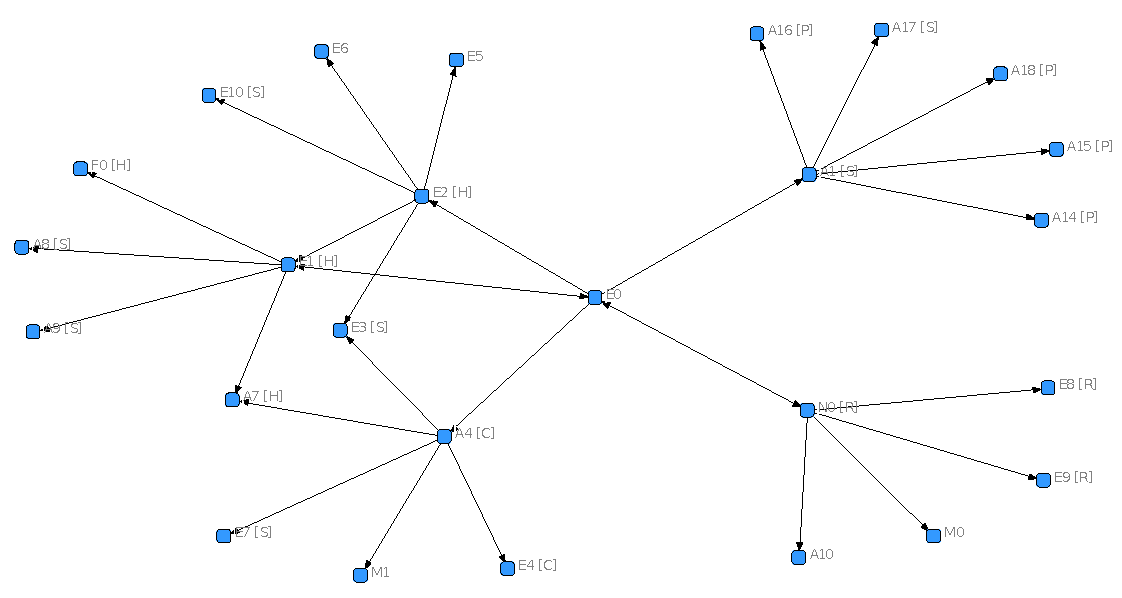
\includegraphics[width=0.8]{figuras/grafo-principal.pdf}}
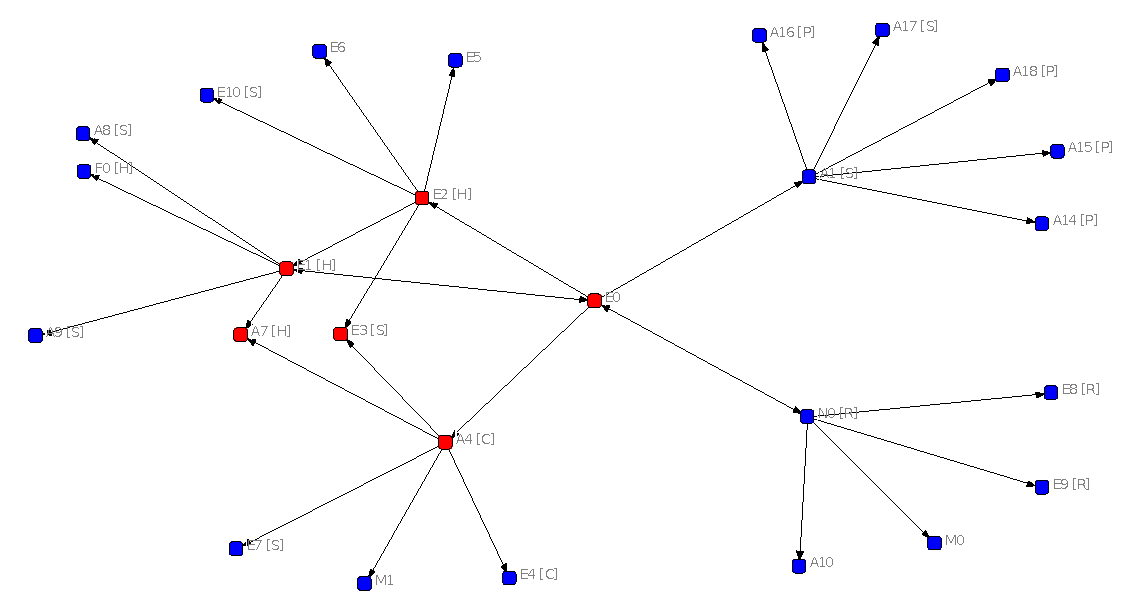
\includegraphics[width=15cm,keepaspectratio]{figuras/grafo-grupos.pdf}
\end{center}

A primeira medida analisada da rede foi a densidade que é a relação entro o número de laços existentes e o número de laços possíveis. Tal métrica exibe a taxa de conectividade. Neste trabalho o valor de densidade encontrado foi de 4,61\% (baixa densidade) o que pode denotar a existência de alguma dificuldade na resolução de problemas em grupo.

Geralmente, nas circunstâncias onde existe baixa densidade, os atores existentes não conseguem se identificar como participantes de um grupo maior e podem demonstrar  dificuldades de relacionamento. Tal situação pode acarretar pouca cooperatividade entres os atores envolvidos, podendo até mesmo existir apatia na resolução de problemas, gerando conflitos. (Hanneman, 2002b).

Alexandra pode completar com a realidade que foi exibida com as entrevistas se contrapondo a ideia do parágrafo anterior.

Outra medida importante é o grau de centralidade, ele indica o número de ligações que entram e que saem de um ator. Através dele são identificados os atores principais da rede. A tabela [] exibe o grau de centralidade associado a cada ator.

\begin{table}[]
\centering
\caption{Grau de centralização de cada ator}
\label{table-centralize-degree}
\begin{tabular}{|l|l|l|l|l|}
\hline
Identificador & Grau de Saída & Grau de Entrada & Grau de Saída  & Grau de Entrada \\ 
	      &               &                 & Normalizada    & Normalizada \\ \hline
E0            & 5,000         & 2,000           & 0,200                     & 0,080                       \\ \hline
A1 {[}S{]}    & 5,000         & 1,000           & 0,200                     & 0,040                       \\ \hline
E1 {[}H{]}    & 5,000         & 2,000           & 0,200                     & 0,080                       \\ \hline
N0 {[}R{]}    & 5,000         & 1,000           & 0,200                     & 0,040                       \\ \hline
A4 {[}C{]}    & 5,000         & 1,000           & 0,200                     & 0,040                       \\ \hline
E2 {[}H{]}    & 5,000         & 1,000           & 0,200                     & 0,040                       \\ \hline
F0 {[}H{]}    & 0,000         & 1,000           & 0,000                     & 0,040                       \\ \hline
A7 {[}H{]}    & 0,000         & 2,000           & 0,000                     & 0,080                       \\ \hline
A8 {[}S{]}    & 0,000         & 1,000           & 0,000                     & 0,040                       \\ \hline
A9 {[}S{]}    & 0,000         & 1,000           & 0,000                     & 0,040                       \\ \hline
A10           & 0,000         & 1,000           & 0,000                     & 0,040                       \\ \hline
E9 {[}R{]}    & 0,000         & 1,000           & 0,000                     & 0,040                       \\ \hline
E8 {[}R{]}    & 0,000         & 1,000           & 0,000                     & 0,040                       \\ \hline
M0            & 0,000         & 1,000           & 0,000                     & 0,040                       \\ \hline
A14 {[}P{]}   & 0,000         & 1,000           & 0,000                     & 0,040                       \\ \hline
A15 {[}P{]}   & 0,000         & 1,000           & 0,000                     & 0,040                       \\ \hline
A16 {[}P{]}   & 0,000         & 1,000           & 0,000                     & 0,040                       \\ \hline
A17 {[}S{]}   & 0,000         & 1,000           & 0,000                     & 0,040                       \\ \hline
A18 {[}P{]}   & 0,000         & 1,000           & 0,000                     & 0,040                       \\ \hline
E10 {[}S{]}   & 0,000         & 1,000           & 0,000                     & 0,040                       \\ \hline
E3 {[}S{]}    & 0,000         & 2,000           & 0,000                     & 0,080                       \\ \hline
E6            & 0,000         & 1,000           & 0,000                     & 0,040                       \\ \hline
E5            & 0,000         & 1,000           & 0,000                     & 0,040                       \\ \hline
E4 {[}C{]}    & 0,000         & 1,000           & 0,000                     & 0,040                       \\ \hline
M1            & 0,000         & 1,000           & 0,000                     & 0,040                       \\ \hline
E7 {[}S{]}    & 0,000         & 1,000           & 0,000                     & 0,040                       \\ \hline
\end{tabular}
\end{table}

Através da tabela [] identifica-se que os principais atores da rede são E0, E1[H], A7 [H] E3[S] pois cada um possui Grau de Entrada Normalizada de 0,8 (mais requisitados).

Alexandra pode falar sobre a importância dos principais atores da rede na resolução de problemas em icapuí.

O Grau de Proximidade denota a capacidade de um ator se ligar a todos os outros atores de uma rede, ou seja, quanto menor a distância entre um ator e outro, maior será seu grau de proximidade. 

Já o Grau de Intermediação mostra a capacidade que um ator possui de intermediar a comunicação entre pares de atores da rede. Sua importância se dá, pois, é através de atores que possuem alto grau de intermediação que as informações são propagadas para diversos outros atores. 

A tabela [closenes] sumariza o Grau de Proximidade e Intermediação dos atores.

\begin{table}[]
\centering
\caption{Grau de Proximidade e Intermediação dos Nós}
\label{closeness-betweeness-degree}
\begin{tabular}{|l|l|l|}
\hline
Identificador & Grau de Proximidade & Grau de Intermediação \\ \hline
E0            & 55.556              & 66.667                \\ \hline
A1 {[}S{]}    & 42.373              & 36.667                \\ \hline
E1 {[}H{]}    & 44.643              & 26.333                \\ \hline
N0 {[}R{]}    & 40.984              & 30.000                \\ \hline
A4 {[}C{]}    & 42.373              & 27.333                \\ \hline
E2 {[}H{]}    & 44.643              & 26.333                \\ \hline
F0 {[}H{]}    & 31.250              & 0.000                 \\ \hline
A7 {[}H{]}    & 35.211              & 2.667                 \\ \hline
A8 {[}S{]}    & 31.250              & 0.000                 \\ \hline
A9 {[}S{]}    & 31.250              & 0.000                 \\ \hline
A10           & 29.412              & 0.000                 \\ \hline
E9 {[}R{]}    & 29.412              & 0.000                 \\ \hline
E8 {[}R{]}    & 29.412              & 0.000                 \\ \hline
M0            & 29.412              & 0.000                 \\ \hline
A14 {[}P{]}   & 30.120              & 0.000                 \\ \hline
A15 {[}P{]}   & 30.120              & 0.000                 \\ \hline
A16 {[}P{]}   & 30.120              & 0.000                 \\ \hline
A17 {[}S{]}   & 30.120              & 0.000                 \\ \hline
A18 {[}P{]}   & 30.120              & 0.000                 \\ \hline
E10 {[}S{]}   & 31.250              & 0.000                 \\ \hline
E3 {[}S{]}    & 35.211              & 2.667                 \\ \hline
E6            & 31.250              & 0.000                 \\ \hline
E5            & 31.250              & 0.000                 \\ \hline
E4 {[}C{]}    & 30.120              & 0.000                 \\ \hline
M1            & 30.120              & 0.000                 \\ \hline
E7 {[}S{]}    & 30.120              & 0.000                 \\ \hline
\end{tabular}
\end{table}

A partir da tabela [closenes] observa-se que os atores E0, A1 [S], E1 [H], N0 [R], A4 [C] e E2 [H] possuem os maiores Graus de Proximidade e os atores E0, A1 [S] e N0 [R] possuem maiores Graus de Intermediação.

Alexandra deve falar como os graus de intermediação e proximidade indicam bem a importância de A1 [S] da Central de Marcação de Consultas e exames.